\chapter{Physical cluster provisioner}
\label{sec:remotevirt}

A resource provisioner is an entity able to provision resources in the form of \gls{slurm} daemons upon request by the \gls{vurm} controller. The \gls{vurm} architecture allows multiple, stackable, resource provisioners and comes with two different implementations. One of them, the physical cluster provisioner, is further described in this chapter.

For additional information about the exact role of a resource provisioner, how it fits into the \gls{vurm} architecture and which tasks it has to be able to accomplish, refer to the \emph{\nameref{sec:architecture}} chapter at page \pageref{sec:architecture}.

The physical cluster provisioner is conceived to manage Linux based HPC clusters. This provisioner is able to execute \gls{slurm} daemons on virtual machines spawned on physical nodes of the cluster and feed them to the \gls{slurm} controller. Additionally this module is also responsible to manage virtual machine migration between physical nodes to better exploit the available computing resources.

The different aspects covered by this chapter are structured as follows:

\begin{itemize}
	\item Section~\ref{sec:cluster-arch} aims to describe the provisioner specific architecture, including the description of both internal and external software components, networking configuration, etc. A class diagram for the overall provisioner architecture is presented as well;
	\item Section~\ref{sec:cluster-deployment} describes all the entities incurring in the deployment of a \texttt{remotevirt} based \gls{vurm} setup;
	\item Section~\ref{sec:libvirt-integration} introduces some \texttt{libvirt} related concepts and conventions and describes the \gls{xml} domain description file used to configure the guests;
	\item Section~\ref{sec:vm-lifecycle} deals with different aspects of the virtual machine lifecycle, such as setup, efficient disk image cloning, different \gls{ip} address retrieval techniques or public key exchange approaches.
\end{itemize}

Aspects directly bound to \gls{vm} migration between physical nodes will not be discussed in this chapter. Refer to the \emph{\nameref{sec:migration}} chapter, starting at page \pageref{sec:migration}, for additional information about this topic.



\section{Architecture}
\label{sec:cluster-arch}

The cluster provisioner takes advantage of the abstraction provided by libvirt to manage \glspl{vm} on the different nodes of the cluster. Each node is thus required to have libvirt installed and the libvirt daemon (\texttt{libvirtd}) running.

Libvirt already implements support for remote management, offering good security capabilities and different client interfaces. Unfortunately, but understandably, the exposed functionalities are strictly virtualization oriented. As the \gls{vurm} cluster provisioner needs to carry out additional and more complex operations on each node individually (IP address retrieval, disk image cloning, \gls{slurm} daemon management,…) an additional component is required to be present on these nodes. This component was implemented in the form of a \gls{vurm} daemon. This daemon exposes the required functionalities and manages the communication with the local libvirt daemon.

An additional \texttt{remotevirt} controller was implemented to centralize the management of the \gls{vurm} daemons distributed on the different nodes. This controller is implemented inside the physical cluster provisioner package and is a completely different entity than the \gls{vurm} controller daemon used to manage resources at an higher abstraction level.

The class diagram in \autoref{fig:remotevirt-arch} on page \pageref{fig:remotevirt-arch} illustrates the whole architecture graphically. The entities on the right (enclosed by the yellow rounded rectangle) are part of the \gls{vurm} daemon running on each single node, while the rest of the entities in the \texttt{vurm.provisioners.remotevirt} package are part of the provisioner interface and the \texttt{remotevirt} controller implementation.

Together with the \texttt{Domain} class, the \texttt{PhysicalNode}, \texttt{VirtualCluster} and \texttt{System} classes allow to model a whole physical cluster, its physical nodes, the various created virtual clusters and their relative domains (virtual nodes).

Each \texttt{PhysicalNode} instance is bound to the remote daemon sitting on the actual computing node by a \texttt{DomainManager} instance. This relationship is also exploited by the \texttt{Domain} instances themselves for operations related to the management of existing \glspl{vm}, as for example \gls{vm} releasing, or (as introduced later on) \gls{vm} migration.

The \texttt{remotevirt} daemons expose a \texttt{DomainManager} instance for remote operations, such as domain creation/destruction and \gls{slurm} daemon spawning. The domain management operations are carried out through a connection to the local libvirt daemon accessed through the bindings provided by the \texttt{libvirt} package. Operations which have to be carried out on the \gls{vm} itself, instead, are executed by exploiting a \gls{ssh} connection provided by the \texttt{SSHClient} object.

More details about the implemented interfaces (\texttt{INode} and \texttt{IProvisioner}) can be found in the \autoref{sec:multiple-provisioners} on page \pageref{sec:multiple-provisioners}, as part of the \emph{\nameref{sec:architecture}} chapter.

The next section offers additional details about how components of this specific provider fit into the global system setup and defines the relationship with other system entities for a correct deployment.

\begin{landscape}
	\begin{figure}
		\centering
		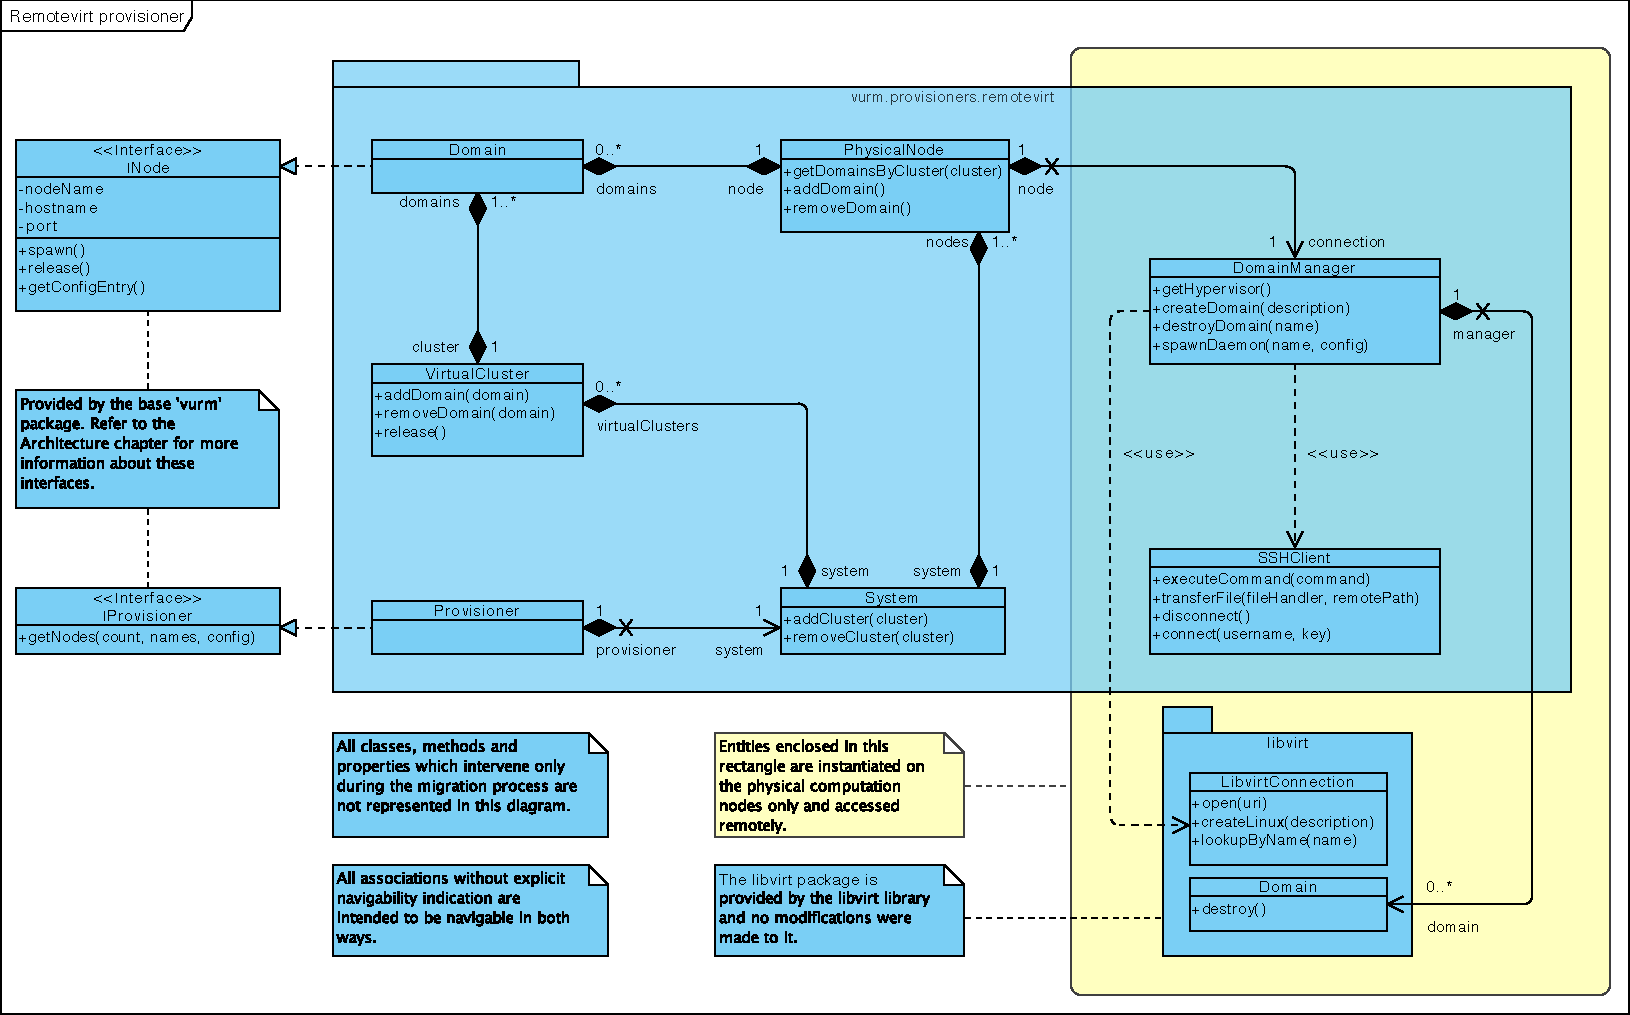
\includegraphics[height=.95\textheight]{figures/remotevirt-provisioner}
		\caption{Overall architecture of the \texttt{remotevirt} provisioner}
		\label{fig:remotevirt-arch}
	\end{figure}
\end{landscape}


\section{Deployment}
\label{sec:cluster-deployment}

The \emph{\nameref{sec:cluster-arch}} section introduced the different entities incurring in the management of \glspl{vm} on a cluster using the \emph{Physical cluster provisioner}. A complete \gls{vurm} system based on this provisioner is even more complex because of the additional components needed to manage the overall virtualized resources.

This section aims to introduce and explain the deployment diagram of a complete \gls{vurm} setup which uses the \emph{Physical cluster provisioner} as its only resource provisioner. All the explications provided in these section refer to the deployment diagram in \autoref{fig:remotevirt-deploy} on page \pageref{fig:remotevirt-deploy}.

The deployment diagram illustrates the most distributed setup currently possible to achieve. All the different logical nodes can be placed on a single physical node if needed (either for testing or development purposes).

For illustration purposes, four different styles were used to draw the different components and artifacts present in the diagram. A legend is available in the bottom left corner of the diagram and defines the coding used for the different formatting styles. The following list provides a more detailed description of the semantics of each style:

\begin{itemize}
	\item The first formatting style was used for externally provided entities which have to be installed by a system administrator and which the \gls{vurm} libraries uses to carry out the different tasks. All these components are provided by either \gls{slurm} or libvirt;
	\item The second formatting style was used for artifacts that the have to be provided either by the system administrator (mainly configuration files) or by the end user (\gls{os} disk images, key pairs,…). The only component in this category is the \texttt{IP address sender}. In the normal case, this component is composed by a small shell script, as described in the subsection~\ref{sec:serial-tcp-ip}. A simple but effective version of this script is provided in the \autoref{lst:serialip};
	\item Components in the third category are provided by the \gls{vurm} library. These components have to be installed by a system administrator in the same way as the \gls{slurm} and libvirt libraries;
	\item The fourth category contains artifacts which are generated at runtime by the different intervening entities. These artifacts don't need to be managed by any third party.
\end{itemize}

The rest of this section is dedicated to explain the role of each represented component in deeper detail.

\subsection*{Commands}

The \texttt{srun}, \texttt{scontrol}, \texttt{valloc} and \texttt{vrelease} components represent either \gls{slurm} or \gls{vurm} commands. As illustrated in the diagram, each command talks directly to the respective entity (the \gls{slurm} controller for \gls{slurm} commands or the \gls{vurm} controller for \gls{vurm} commands). This difference is abstracted from the user perspective and does not involve additional usage complexity.

Additional, not illustrated, commands may be available. The \gls{slurm} library comes with a plethora of additional commands, such as \texttt{sview}, \texttt{sinfo}, \texttt{squeue}, \texttt{scancel}, etc.

\subsection*{\texttt{VurmController} and \texttt{RemotevirtProvisioner}}

The \texttt{VurmController} component represents the \gls{vurm} controller daemon, configured with the \texttt{RemotevirtProvisioner}. The provisioner component represents both the \texttt{IProvisioner} realization itself and the \texttt{remotevirt} controller introduced in the previous section. The user manual in the \autoref{apx:user-manual} offers a complete reference for this configuration file.

Both the entities can be configured through a single \emph{\gls{vurm} configuration file}. This file contains the configuration for the overall \gls{vurm} system and also defines the different physical nodes available to the \texttt{remotevirt} provisioner.

\subsection*{Domain description file}

The domain description file is used as a template to generate an actual domain description to pass to the \gls{vurm} daemons. This file describes a libvirt domain using an \gls{xml} syntax defined by libvirt itself. The \autoref{sec:libvirt-integration} offers an overview of the different available elements, describes the additions made by \gls{vurm} and presents part of the default domain description file.

\subsection*{\texttt{VurmdLibvirt}, \texttt{Libvirt} and \texttt{KVM/QEMU}}

The three components placed on the physical node are responsible to carry out the management operations requested by the controller. Despite being represented one single time on the deployment diagram, a \gls{vurm} system using the \texttt{remotevirt} provisioner normally consists of one controller node and many different physical nodes. The same argument can be made for the virtual node too: a physical node is able to host different virtual nodes.

The \texttt{VurmdLibvirt} component mainly offers a facade for more complex operations over the \texttt{libvirt} daemon and is responsible for the local housekeeping of the different assets (mainly disk image clones and state files). The \texttt{libvirt} daemon and the hypervisor of choice, in this case \texttt{KVM/QEMU}, are used to effectively create, destroy and migrate the \glspl{vm} themselves.

The particular port between the \texttt{VurmdLibvirt} and the \texttt{IP address sender} components is needed to get the \gls{ip} address from the \gls{vm} once it is assigned to it. The used \gls{ip} address retrieval technique is described in deeper detail in the \autoref{sec:ip-address-retrieval}.

\subsection*{AMP protocol}

The \gls{slurm} commands talk to the \gls{slurm} controller by using a custom \gls{slurm} binary protocol, while the \gls{vurm} commands adopt the \gls{amp} protocol. The same protocol is also adopted by the \texttt{remotevirt} provisioner to communicate with the daemons placed on each single node.

\gls{amp} \cite{amp-www} is an asynchronous key/value pair based protocol with implementations in different languages. The asynchronous nature of \gls{amp} allows to send multiple request/response pairs over the same connection and without having to wait to obtain a response to a previous request before sending a new one.

The adoption of \gls{amp} as the default protocol to communicate between the \gls{vurm} entities allows to reach an higher degree of scalability thanks to the reuse and multiplexing of different channels over a single TCP/IP connection.

\begin{landscape}
	\begin{figure}
		\centering
		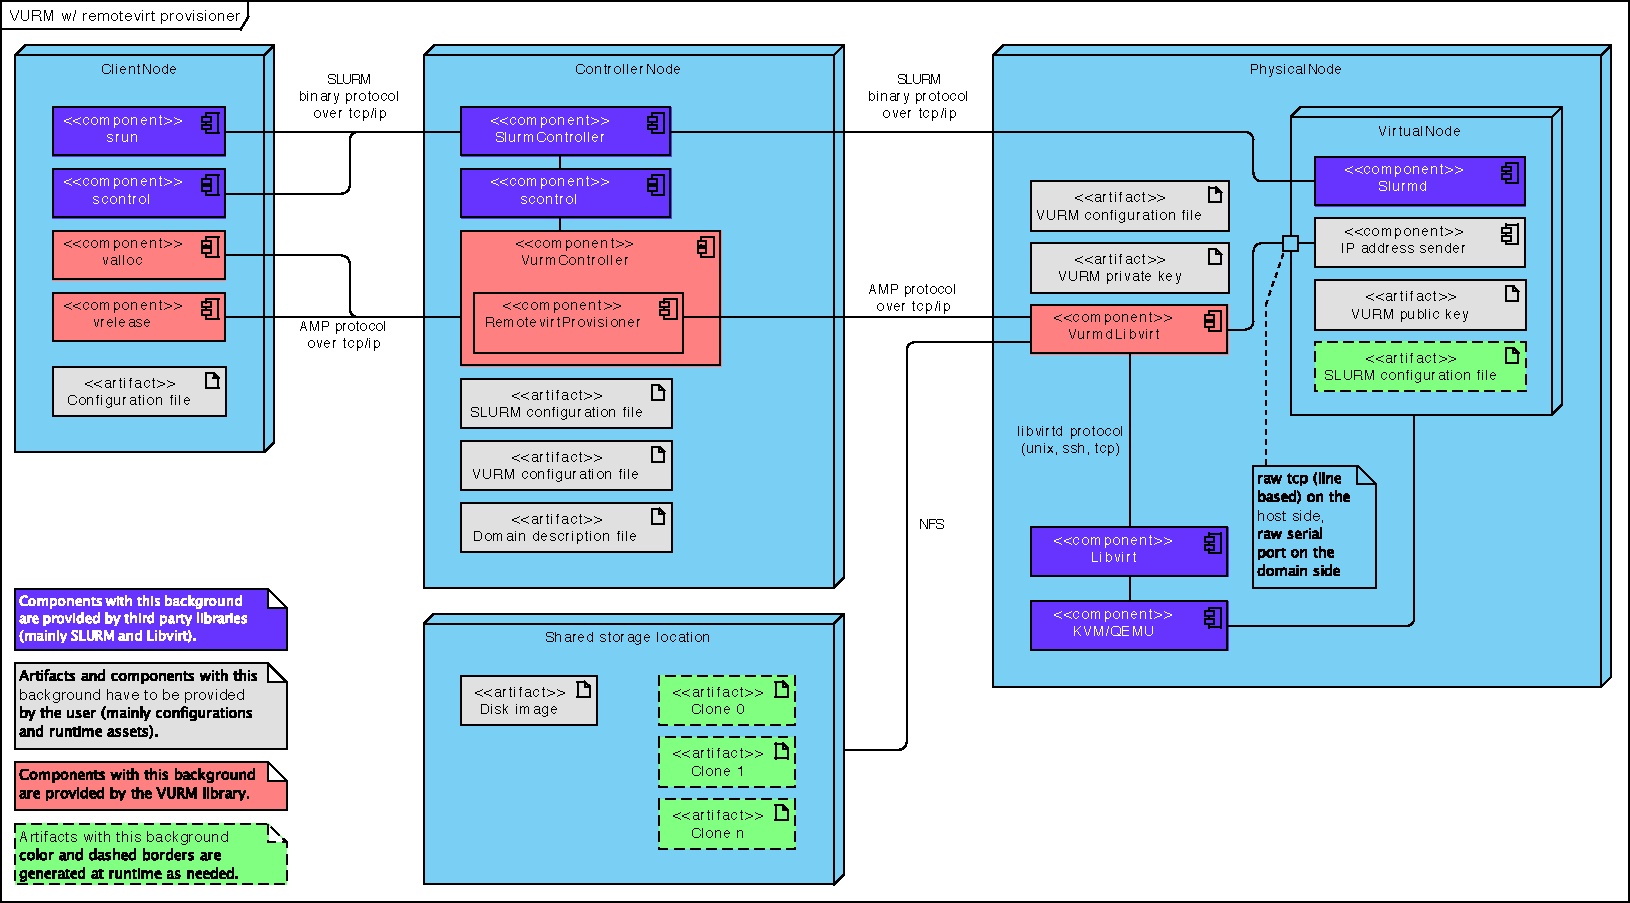
\includegraphics[height=.85\textheight]{figures/cluster-deployment}
		\caption{Complete VURM + remotevirt deployment diagram}
		\label{fig:remotevirt-deploy}
	\end{figure}
\end{landscape}


\section{Libvirt integration}
\label{sec:libvirt-integration}

The libvirt library provides an abstraction layer to manage virtual machines by using different hypervisors, both locally and remotely. It offers an \gls{api} to create, start, stop, destroy and otherwise manage virtual machines and their respective resources such as network devices, storage devices, processor pinnings, hardware interfaces, etc. Additionally, through the libvirt daemon, it accepts incoming remote connections and allows complete exploitation of the \gls{api} from remote locations, while accounting for authentication and authorization related issues.

The libvirt codebase is written in C, but bindings for different languages are provided as part of the official distribution or as part of external packages. The currently supported languages are C, C\#, Java, OCaml, Perl, PHP, Python and Ruby. For the scope of this project the Python bindings were used.

Remote connections can be established using raw \gls{tcp}, \gls{tls} with x509 certificates or \gls{ssh} tunneling. Authentication can be provided by Kerberos and \gls{sasl}. Authentication of local connections (using unix sockets) can be controlled with PolicyKit.

To abstract the differences between \gls{vm} management over different hypervisors, libvirt adopts a special naming convention and defines its own \gls{xml} syntax to describe the different involved resources. This section aims to introduce the naming convention, and the \gls{xml} description file. The \gls{xml} description file subsection includes the explications of the changes introduced by the \gls{vurm} virtualization model.


\subsection{Naming conventions}

Libvirt adopts the following naming conventions to describe the different entities involved in the \gls{vm} lifecycle:

\begin{itemize}
	\item A \emph{node} is a single physical machine;
	\item An \emph{hypervisor} is a layer of software allowing to virtualize a node in a set of virtual machines with possibly different configurations than the node itself;
	\item A \emph{domain} is an instance of an operating system running on a virtualized machine provided by the hypervisor.
\end{itemize}

Under this naming convention and for the scope of the \gls{vurm} project, the definition of \gls{vm} or of \emph{virtual node} is thus the same as the definition of \emph{domain}.


\subsection{XML description file}

The \gls{xml} description file is the base for the definition of a new domain. This file contains all needed information, such as memory allocation, processor pinning, hypervisor features to enable, disks definition, network interfaces definitions, etc.

Given the wide range of configuration options to support, a complete description of the available elements would be too long to include in this section. The complete reference is available online at \cite{libvirt-domains}. For the purposes of this project, the description of the elements contained in the \gls{xml} description presented in \autoref{lst:libvirtxml} is more than sufficient.

\lstset{language=xml,caption=Basic libvirt XML description file,label=lst:libvirtxml}
\begin{lstlisting}
<domain type="kvm">
	<name>domain-name</name>

	<memory>1048576</memory>

	<vcpu>2</vcpu>

	<os>
		<type arch="x86_64">hvm</type>
		<boot dev="hd"/>
	</os>

	<features>
		<acpi/>
		<hap/>
	</features>

	<devices>
		<emulator>/usr/bin/qemu-system-x86_64</emulator>

		<disk type="file">
			<driver name="qemu" type="qcow2"/>
			<source file="debian-base.qcow2"/>
			<target dev="sda" bus="virtio"/>
		</disk>

		<interface type="bridge">
			<source bridge="br0"/>
			<target dev="vnet0"/>
			<model type='virtio'/>
		</interface>
	</devices>
</domain>
\end{lstlisting}

The root element for the definition of a new domain is the \texttt{domain} element. Its \texttt{type} attribute identifies the hypervisor to use.

Each \texttt{domain} element has a \texttt{name} element containing a host-unique name to assign to the newly spawned \gls{vm}. When using the remotevirt provisioner to spawn new virtual machines, the name element will automatically be set (and overridden if present).

The \texttt{memory} element contains the amount of memory to allocate to this domain. The units of this value are kilobytes. In this case, $1GB$ of memory is allocated to the domain.

The \texttt{type} child of the \texttt{os} element specifies the type of operating system to be booted in the virtual machine. \texttt{hvm} indicates that the \gls{os} is one designed to run on bare metal, so requires full virtualization. The optional \texttt{arch} attribute specifies the \glstext{cpu} architecture to virtualize.

The \texttt{features} element can be used to enable additional features. In this case the \texttt{acpi} (useful for power management, for example, with KVM guests it is required for graceful shutdown to work) and \texttt{hap} (enables use of Hardware Assisted Paging if available in the hardware) features are enabled.

The content of the \texttt{emulator} element specifies the fully qualified path to the device model emulator binary to be used.

The \texttt{disk} element is the main container for describing disks. The \texttt{type} attribute is either \texttt{file}, \texttt{block}, \texttt{dir}, or \texttt{network} and refers to the underlying source for the disk. The optional \texttt{device} attribute indicates how the disk is to be exposed to the guest \gls{os}. Possible values for this attribute are \texttt{floppy}, \texttt{disk} and \texttt{cdrom}, defaulting to \texttt{disk}.

The \texttt{file} attribute of the \texttt{source} element specifies the fully-qualified path to the file holding the disk. The path contained by this attribute is always resolved as a child of the path defined by the \texttt{imagedir} option in the \gls{vurm} configuration (in the case of a \gls{vurm} setup, absolute path are thus not supported).

The optional \texttt{driver} element allows specifying further details related to the hypervisor driver used to provide the disk. QEMU/KVM only supports a name of \texttt{qemu}, and multiple types including \texttt{raw}, \texttt{bochs}, \texttt{qcow2}, and \texttt{qed}.

The \texttt{target} element controls the bus/device under which the disk is exposed to the guest OS. The \texttt{dev} attribute indicates the logical device name. The optional \texttt{bus} attribute specifies the type of disk device to emulate; possible values are driver specific, with typical values being \texttt{ide}, \texttt{scsi}, \texttt{virtio}, \texttt{xen} or \texttt{usb}.



\section{VM Lifecycle aspects}
\label{sec:vm-lifecycle}

Before being able to run the \gls{slurm} daemon, different operations have to be performed. The ultimate goal of this set of operations if to have a \gls{vm} up and running. This section aims to describe the different involved steps to reach this goal and to discuss some alternative approaches for some of them.

The sequence diagram in \autoref{fig:domain-lifecycle} on page \pageref{fig:domain-lifecycle} illustrates the complete \gls{vm} lifecycle. The lifecycle can be divided in three phases: the first phase (domain creation) occurs when the creation request is first received, the second phase (\gls{slurm} daemon spawning) occurs as soon as all domains of the virtual cluster were correctly created and the \gls{ip} addresses received and the third phase (domain destruction) occurs once that the end-user finished to execute \gls{slurm} jobs on the virtual cluster and asks for it to be released.

Two operations of the first phase, more precisely the messages 1.1 and 1.3, deserve some particular attention. The subsections \ref{sec:ip-address-retrieval} and \ref{sec:volumes-cloning} address these operations respectively.

The last subsection is dedicated to explain some of the possible public-key exchange approaches needed to perform a successful authentication when connecting to the \gls{vm} through \gls{ssh} (message 3.1). Due to the nature of the adopted solution, no messages are visible on the diagram for this operation.


\subsection{IP address retrieval}
\label{sec:ip-address-retrieval}

The simplest way to interact with a newly started guest is through a TCP/IP connection. The \gls{vurm} tools use \gls{ssh} to execute commands on the guest, while the \gls{slurm} controller communicates with its daemons over a socket connection. All of these communications means require the \gls{ip} address (or the hostname) of the guest to be known.

At present, \texttt{libvirt} does not exposes any \glspl{api} to retrieve a guests \gls{ip} address and a solution to overcome this shortcoming has to be implemented completely by the calling codebase.

During the execution of the project, different methods were analyzed and compared; the rest of this sub section is dedicated to analyze the advantages and shortcomings of each of them.

\subsubsection{Inspect host-local ARP tables}

As soon as a guest establish a \gls{tcp} connection with the outside world, it has to advertise its \gls{ip} address in an \gls{arp} response. This causes the other hosts on the same subnet to pick it up and cache it in its \gls{arp} table.

Running the \texttt{arp -an} command on the host will reveal the contents of the \gls{arp} table, as presented in \autoref{lst:arp}:

\lstset{language=bash,caption=Example \texttt{arp -an} output,label=lst:arp}
\begin{lstlisting}
$ arp -an
? (10.0.0.1) at 0:30:48:c6:35:ea on en0 ifscope [ethernet]
? (10.0.0.95) at 52:54:0:48:5c:1f on en0 ifscope [ethernet]
? (10.0.1.101) at 0:14:4f:2:59:ae on en0 ifscope [ethernet]
? (10.0.6.30) at 52:54:56:0:0:1 on en0 ifscope [ethernet]
? (10.255.255.255) at ff:ff:ff:ff:ff:ff on en0 ifscope [ethernet]
? (129.24.176.1) at 0:1c:e:f:7c:0 on en1 ifscope [ethernet]
? (129.24.183.255) at ff:ff:ff:ff:ff:ff on en1 ifscope [ethernet]
? (169.254.255.255) at (incomplete) on en0 [ethernet]
\end{lstlisting}

As libvirt is able to retrieve the \gls{mac} address associated with a given interface, it is possible to parse the output and retrieve the correct \gls{ip} address.

This method could not be adopted because \gls{arp} packets do not pass across routed networks and the bridged network layout used by the spawned domains would thus stop them.

\subsubsection{Proprietary VM Tools}

Some hypervisors (as, for example, VMWare ESXi or VirtualBox), are coupled with a piece of software which can be installed on the target guest and provides additional interaction capabilities, such as commands execution, enhanced virtual drivers or, in this case, \gls{ip} address retrieval.

Such a tool would bind the whole system to a single hypervisor and would vanish the efforts done to support the complete range of libvirt-compatible virtual machine monitors. Additionally, the KVM/Qemu pair, chosen for their live migration support, does not provide such a tool.

\subsubsection{Static DHCP entries}

A second possible method is to configure a pool of statically defined \gls{ip}/\gls{mac} address couples in the \gls{dhcp} server and configure the \gls{mac} address in the libvirt \gls{xml} domain description file in order to know in advance which \gls{ip} address will be assigned to the \gls{vm}.

This method could have worked and is a viable alternative; it was however preferred to not depend on external services (the \gls{dhcp} server, in this case) and provide a solution which can work in every context. A configuration switch to provide a list of \gls{ip}/\gls{mac} address pairs instead of the adopted solution can although be considered as a future improvement.

\subsubsection{Serial to TCP data exchange}
\label{sec:serial-tcp-ip}

The last explored and successfully adopted method takes advantage of the serial port emulation feature provided by the different hypervisors and the capability to bind them to (or connect them with) a \gls{tcp} endpoint of choice.

In the actual implementation, the \gls{vurm} daemon listens on a new (random) port before it spawns a new \gls{vm}; the libvirt daemon will then provide a serial port to the guest and connect it to the listening server. Once booted, a little script on the guest writes the IP address to the serial port and the \gls{tcp} server receives it as a normal TCP/IP data stream.

Although not authenticated nor encrypted, this communication channel is deemed secure enough as no other entity can possibly obtain relevant information by eavesdropping the communication (only an \gls{ip} address is exchanged). Additionally, as it's the hypervisor task to establish the \gls{tcp} connection directly to the local host, there is no danger for man-in-the-middle attacks (and thus invalid information being transmitted).\footnote{The daemon only binds to the loopback interface; a malicious process should be running on the same host to possibly connect to the socket and send a wrong \gls{ip} address}
The \autoref{lst:serialtcp} contains the needed libvirt device configuration:

\lstset{language=xml,caption=Libvirt TCP to serial port device description,label=lst:serialtcp}
\begin{lstlisting}
<serial type="tcp">
    <source mode="connect" host="127.0.0.1" service="$PORT"/>
    <protocol type="raw"/>
    <target port="1"/>
    <alias name="serial0"/>
</serial>
\end{lstlisting}

The shell script on the guest needed to write the \gls{ip} address to the serial device can be as simple as the following:

\lstset{language=bash,caption=Shell script to write the \gls{ip} address to the serial port,label=lst:serialip}
\begin{lstlisting}
#!/bin/sh
ifconfig eth0 | grep -oE '([0-9]{1,3}\.){3}[0-9]{1,3}' | head -1 >/dev/ttyS0
\end{lstlisting}


\subsection{Volumes cloning}
\label{sec:volumes-cloning}

During the virtual cluster creation phase, the user has the possibility to choose which disk image all the created \glspl{vm} will be booted from.

As a virtual cluster is formed by multiple \glspl{vm}, and as each virtual machine needs its own disk image from which read from and to which write to, multiple copies of the base image have to be created.

Performing a raw copy of the base image presents obvious limitations: firstly each copy occupies the same amount of space as the original image, which rapidly leads to fill up the available space on the storage device, and secondly, given the necessity of these images to live on a shared file system (see \autoref{sec:migration} for the details), the copy operation can easily fill up the available network bandwidth and take a significant amount of time.

To overcome these drawbacks, a particular disk image format called \gls{qcow2} is used. This particular format has two useful features:

\begin{itemize}
    \item A \texttt{qcow2} image file, unlike a \texttt{raw} disk image, occupies only the equivalent of the size of the data effectively written to the disk. This means that it is possible to create a 40GB disk image which, once a base \gls{os} is installed on it, occupies only a couple of GBs\footnote{Other disk image formats support this feature too. For example \texttt{qcow} (version 1) or \texttt{VMDK} (when using the \texttt{sparse} option).};
    \item It is possible to create a disk image based on another one. Read data is retrieved from the base image until the guest modifies it. Modified data is written only to the new image, while leaving the base image intact. The \autoref{fig:cow} represents this process graphically.
\end{itemize}

\begin{figure}[h]
	\centering
	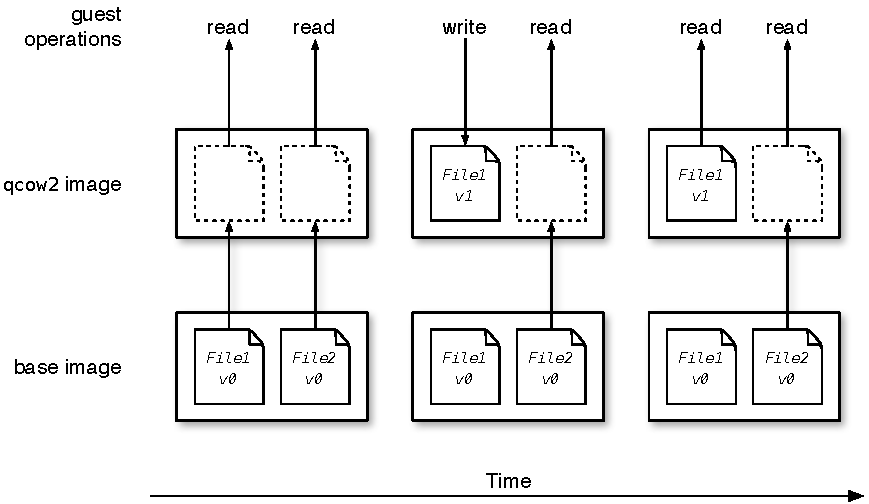
\includegraphics[width=0.6\textwidth]{figures/cow-images}
	\caption{Copy-On-Write image R/W streams}
	\label{fig:cow}
\end{figure}

The combination of these two features allows to create per-VM disk images in both a time- and space-efficient manner.



\subsection{Public key exchange}
\label{sec:pk-exchange}

As anticipated in \autoref{sec:cluster-arch}, the \gls{vurm} daemon executes commands on the guest through a \gls{ssh} connection. The daemon authentication modes were deliberately restricted, for security reasons, to public key authentication only.

This restriction requires that the daemon public key is correctly installed on the guest disk image. As the disk image is customizable by the user, it is necessary to define how this public key will be installed.

Different techniques can be used to achieve this result; the rest of this subsection is dedicated to analyze three of them.

\subsubsection{Public key as a requirement}

The simplest (from the \gls{vurm} point of view) solution is to set the setup of a \gls{vurm}-specific user account with a given public key as a requirement to run a custom disk image on a given \gls{vurm} deployment.

This approach requires the end user to manually configure its custom disk image. The obvious drawback is the inability to run the same disk image on different \gls{vurm} deployments as the key pair differs from setup to setup.\footnote{This is, however, a very minor drawback; the percentile of users running jobs on different clusters is very low, and even so, the disk image probably needs adjustments of other parameters anyway.}

The final chosen solution is based on this approach, given that the disk image has to be specifically customized because of other parameters anyway. Refer to the \autoref{sec:vm-creation} in the \emph{\nameref{apx:user-manual}} for more information about the \gls{vm} disk image creation process.

\subsubsection{Pre-boot key installation}

Another explored technique consists of mounting the disk image on the host, copying the public key to the correct location, unmounting the image and then starting the guest.

The mounting, copying and unmounting operation was made straightforward by the use of a specific image manipulation library called \texttt{libguestfs}.

For security reasons, this library would spawn a new especially crafted VM instead of mounting the image directly on the host; this made the whole key installation operation a long task when compared with the simplicity of the problem (mounting, copying and unmounting took an average of 5 seconds during the preliminary tests).

The poor performances of the operation, its different dependencies (too many for such a simple operation) and its tight coupling with the final public key path on the guest, led this approach to be discarded in the early prototyping phase.

\subsubsection{IP-Key exchange}

As seen in the previous section, the final solution adopted to retrieve a guest IP address, already requires to setup a communication channel between the \gls{vurm} daemon and the guest.

The idea of this approach is to send back the public key to the guest as soon as the IP address is received. In this case, the guest would first write the \gls{ip} address to the serial port and then read the public key and store it to the appropriate location. An extension to the shell script \ref{lst:serialip} which saves the public key as a valid key to login as root is presented in the \autoref{lst:serialip2}:

\lstset{language=bash,caption=Shell script to exchange the IP address and a public key over the serial port,label=lst:serialip2}
\begin{lstlisting}
#!/bin/sh
ifconfig eth0 | grep -oE '([0-9]{1,3}\.){3}[0-9]{1,3}' | head -1 >/dev/ttyS0
mkdir -p /root/.ssh
chmod 0755 /root/.ssh
cat /dev/sttyS0 >>/root/.ssh/authorized_keys
chmod 0644 /root/.ssh/authorized_keys
\end{lstlisting}

This technique was firstly adopted, but then discarded in favor of the more proper requirement-based solution as bidirectional communication using a serial port revealed to be too complicated to implement correctly in a simple shell script.\footnote{Synchronization and timing issues which could not simply be solved by using timeouts where detected when running slow guests.}

A proper solution would have required the installation of a custom built utility; copying a simple file (the public key) was considered a less troublesome operation than installing yet another utility along with its dependencies.


\section{Possible improvements}
\label{sec:future-cluster}

\subsection{Disk image transfer}

The current implementation takes advantage of the \gls{nfs} support already required by libvirt\footnote{\gls{nfs} support is required by libvirt and the qemu driver for \gls{vm} migration, more details are given in the \autoref{sec:migration}.} to exchange disk images between the controller and the physical nodes. On clusters consisting of many nodes, the shared network location becomes a bottleneck as soon as multiple daemons try to access the same disk image to start new \glspl{vm}.

A trivial improvement would consist of a basic file exchange protocol allowing to transfer the disk image between the controller and the daemons while optimizing and throttling this process in order to not saturate the whole network.

As well as the \gls{nfs} based solution, the trivial approach also exposes different and non-negligible drawbacks and can be further optimized. The nature of the task -- distributing a single big file to a large number of entities -- seems to be a perfect fit for the BitTorrent protocol, as better highlighted in the official protocol specification \cite{bittorrent-www}:

\begin{quote}
BitTorrent is a protocol for distributing files. \emph{[…]} Its advantage over plain HTTP is that when multiple downloads of the same file happen concurrently, the downloaders upload to each other, making it possible for the file source to support very large numbers of downloaders with only a modest increase in its load.
\end{quote}

A more advanced and elegant solution would thus implement disk image transfers using the BitTorrent protocol instead of a more traditional \emph{single-source} distribution methodology.

\subsection{Support for alternative VLAN setups}

The current implementations bridges the \gls{vm} network connection directly to the physical network card of the host system. \glspl{vm} appear thus on the network as standalone devices and they share the same subnet as their hosts.

It could be possible to create an isolated \gls{vlan} subnet for each virtual cluster in order to take advantage of the different aspects offered by such a setup, as for example, traffic control patterns and quick reactions to inter-subnet relocations (useful in case of \gls{vm} migrations).

This improvement would add even more flexibility to the physical cluster provisioner and enable even more transparent \gls{slurm} setups spawning multiple clusters residing in different physical locations.

It is useful to note that different private cloud managers already implement and support \gls{vlan} setups to various degrees (the example par excellence being Eucalyptus \cite{eucalyptus-manual} \cite{eucalyptus-ns-www}).


\begin{figure}[p]
	\centering
	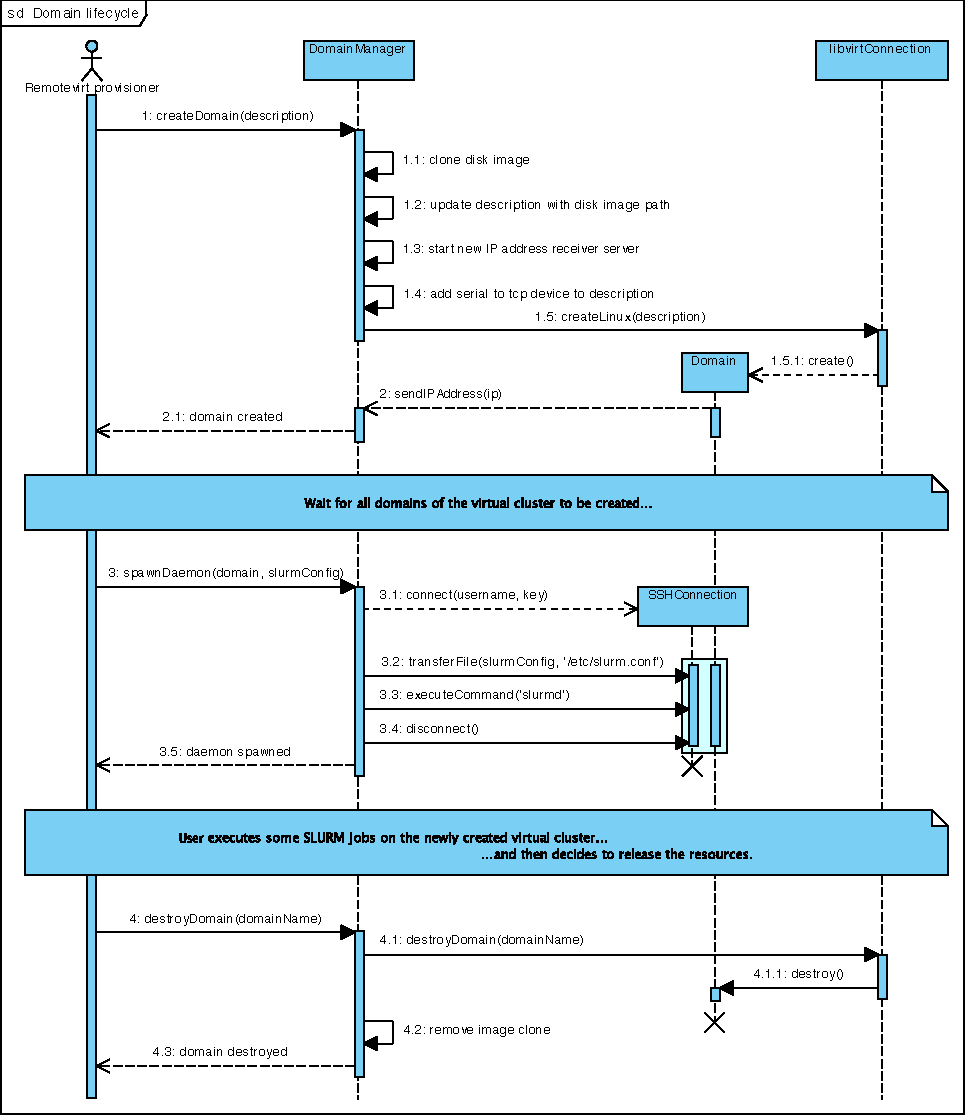
\includegraphics[width=1\textwidth]{figures/domain-lifecycle}
	\caption{Complete domain lifecycle}
	\label{fig:domain-lifecycle}
\end{figure}